\documentclass[journal]{IEEEtran}
%\documentclass[12pt, draftclsnofoot, onecolumn]{IEEEtran}

\usepackage{cite}
\usepackage{amsmath,amssymb,amsfonts}
\usepackage{algorithm}
\usepackage{algorithmic}
\usepackage{graphicx}
\usepackage{textcomp}
\usepackage{xcolor}
\usepackage{color}
\usepackage{bm}
\usepackage{subfigure}

% *** GRAPHICS RELATED PACKAGES ***
%
\ifCLASSINFOpdf
  % \usepackage[pdftex]{graphicx}
  % declare the path(s) where your graphic files are
  % \graphicspath{{../pdf/}{../jpeg/}}
  % and their extensions so you won't have to specify these with
  % every instance of \includegraphics
  % \DeclareGraphicsExtensions{.pdf,.jpeg,.png}
\else
  % or other class option (dvipsone, dvipdf, if not using dvips). graphicx
  % will default to the driver specified in the system graphics.cfg if no
  % driver is specified.
  % \usepackage[dvips]{graphicx}
  % declare the path(s) where your graphic files are
  % \graphicspath{{../eps/}}
  % and their extensions so you won't have to specify these with
  % every instance of \includegraphics
  % \DeclareGraphicsExtensions{.eps}
\fi
% graphicx was written by David Carlisle and Sebastian Rahtz. It is
% required if you want graphics, photos, etc. graphicx.sty is already
% installed on most LaTeX systems. The latest version and documentation
% can be obtained at: 
% http://www.ctan.org/pkg/graphicx
% Another good source of documentation is "Using Imported Graphics in
% LaTeX2e" by Keith Reckdahl which can be found at:
% http://www.ctan.org/pkg/epslatex
%
% latex, and pdflatex in dvi mode, support graphics in encapsulated
% postscript (.eps) format. pdflatex in pdf mode supports graphics
% in .pdf, .jpeg, .png and .mps (metapost) formats. Users should ensure
% that all non-photo figures use a vector format (.eps, .pdf, .mps) and
% not a bitmapped formats (.jpeg, .png). The IEEE frowns on bitmapped formats
% which can result in "jaggedy"/blurry rendering of lines and letters as
% well as large increases in file sizes.
%
% You can find documentation about the pdfTeX application at:
% http://www.tug.org/applications/pdftex




% *** ALIGNMENT PACKAGES ***
%
%\usepackage{array}
% Frank Mittelbach's and David Carlisle's array.sty patches and improves
% the standard LaTeX2e array and tabular environments to provide better
% appearance and additional user controls. As the default LaTeX2e table
% generation code is lacking to the point of almost being broken with
% respect to the quality of the end results, all users are strongly
% advised to use an enhanced (at the very least that provided by array.sty)
% set of table tools. array.sty is already installed on most systems. The
% latest version and documentation can be obtained at:
% http://www.ctan.org/pkg/array


% IEEEtran contains the IEEEeqnarray family of commands that can be used to
% generate multiline equations as well as matrices, tables, etc., of high
% quality.



% *** Do not adjust lengths that control margins, column widths, etc. ***
% *** Do not use packages that alter fonts (such as pslatex).         ***
% There should be no need to do such things with IEEEtran.cls V1.6 and later.
% (Unless specifically asked to do so by the journal or conference you plan
% to submit to, of course. )


% correct bad hyphenation here
\hyphenation{op-tical net-works semi-conduc-tor}


\begin{document}
%
% paper title
% Titles are generally capitalized except for words such as a, an, and, as,
% at, but, by, for, in, nor, of, on, or, the, to and up, which are usually
% not capitalized unless they are the first or last word of the title.
% Linebreaks \\ can be used within to get better formatting as desired.
% Do not put math or special symbols in the title.
\title{Resource Allocation for Intelligent Reflecting Surface Aided Vehicular Communications}
%
%
% author names and IEEE memberships
% note positions of commas and nonbreaking spaces ( ~ ) LaTeX will not break
% a structure at a ~ so this keeps an author's name from being broken across
% two lines.
% use \thanks{} to gain access to the first footnote area
% a separate \thanks must be used for each paragraph as LaTeX2e's \thanks
% was not built to handle multiple paragraphs
%

\author{Yuanbin~Chen,~Ying~Wang,~\IEEEmembership{Member,~IEEE,}
        Jiayi~Zhang,~\IEEEmembership{Senior Member,~IEEE,}~and~Zhendong~Li% <-this % stops a space
\thanks{Copyright (c) 2015 IEEE. Personal use of this material is permitted. However, permission to use this material for any other purposes must be obtained from the IEEE by sending a request to pubs-permissions@ieee.org.
	
	This work is supported by National Key Research and Development Program of China (2017YFE0120600). \textit{(Corresponding author: Ying Wang.)}
	
	Y. Chen, Y. Wang and Z. Li are with State Key Laboratory of Networking and Switching Technology, Beijing University of Posts and Telecommunications, Beijing, China 100876 (e-mail: chen\_yuanbin@163.com; wangying@bupt.edu.cn; ielizhendong@163.com).
	
J. Zhang is with the School of Electronic and Information Engineering, Beijing Jiaotong University, Beijing 100044, China (e-mail: jiayizhang@bjtu.edu.cn).}% <-this % stops a space
% <-this % stops a space
}


% make the title area
\maketitle

% As a general rule, do not put math, special symbols or citations
% in the abstract or keywords.
\begin{abstract}
%As an emerging and promising technology, intelligent reflecting surface (IRS) can significantly enhance wireless conmmunication by intelligently reflecting the received signal. 
%Due to the fact that high mobility of vehicles and the complicated propagation environment pose major challenge to vehicular communications, intelligent reflecting serface (IRS) aided vehicular communications is of great significance.
This paper studies the resource allocation for intelligent reflecting surface aided vehicular communications based on slowly varying large-scale fading channel information. To meet different quality-of-service (QoS) requirements of vehicular communications, we aim to maximize the sum vehicle-to-infrastructure (V2I) link capacity while guaranteeing the minimum signal-to-interference-plus-noise ratio (SINR) of vehicle-to-vehicle (V2V) links. More specifically, the power allocation, IRS reflection coefficients and spectrum allocation are jointly optimized. To tackle the formulated mixed integer non-convex problem, we divide it into two stages, which yields an alternating optimization algorithm. Simulation results demonstrate the effectiveness of the proposed algorithm and the IRS can significantly improve the quality of vehicular communications in terms of the sum V2I capacity.
\end{abstract}

% Note that keywords are not normally used for peerreview papers.
\begin{IEEEkeywords}
Intelligent reflecting surface, resource allocation, vehicular communications, alternating optimization.
\end{IEEEkeywords}


\section{Introduction}

The emergence of vehicle-to-everything (V2X) communications aims to make people's daily travels safer and more convenient, thereby paving the way for cutting-edge intelligent applications, such as intelligent transportation systems and autonomous driving. However, due to the complicated propagation environment, especially considering the occlusion of multiple buildings in urban areas and the fast varying channels caused by the high mobility of vehicles, the propagation links of vehicular communications are easily deteriorated. In order to improve the quality of vehicular communications, intelligent reflecting surface (IRS) has attracted widespread attention in enhancing wireless transmission \cite{IRS-1,zhang1,song}. 

IRS-aided wireless communication systems have been extensively studied in the literature, such as IRS-aided  unmanned aerial vehicle (UAV) system~\cite{IRS-3}, IRS-aided simultaneous wireless information and power transfer (SWIPT) system~\cite{IRS-A-12}, etc. Nevertheless, the research on resource management of IRS-aided wireless communication is still in its infancy. It was investigated in~\cite{IRS-A-9} that the IRS phase shift matrix and power allocation are jointly optimized. The joint optimization of the IRS reflection coefficients together with the orthogonal frequency division multiple access (OFDMA) time-frequency resource block and power allocations was studied in~\cite{IRS-12}. Given the complicated propagation environment of vehicular communications and the high mobility of vehicles \cite{zhang2}, the IRS can smartly control the radio environment to improve the communication quality and enlarge the signal coverage with its low cost and high energy-efficiency. However, its reflection coefficients need to be jointly optimized with multi-vehicle transmission scheduling and spectrum allocation. Therefore, it is necessary to design the resource allocation algorithm to guarantee the quality-of-service (QoS) of each V2X communication link. To the best of our knowledge, this is the first work on the design of IRS-aided vehicular communications.
%The IRS consists of a large number of reconfigurable passive elements, and each element can  reflect the received signal independently by adjusting the reflection coefficients (including phase shift and amplitude), thereby strengthening the power of the received signal at the receiver. Different from traditional relays and large-scale multiple input multiple output (MIMO) based on active intelligent surfaces, the IRS has lower power consumption and implementation cost, which allows IRS to yield superior performance by increasing the number of elements with affordable hardware cost and tolerateble power consumption~\cite{IRS-2}.


Against the above background and inspired by the superiority of deploying the IRS in vehicular networks to improve the quality of V2X communications, in this paper, we consider the resource allocation for IRS-aided vehicular communications, where vehicle-to-vehicle (V2V) and vehicle-to-infrastructure (V2I) links with different QoS requirements share spectrum. Specifically, resource allocation is based on large-scale slowly varying channel statistics instead of instantaneous channel state information (CSI), which embraces the challenging brought by high mobility. To incorporate and satisfy different QoS requirements of applications carried by different types of connections, we aim to maximize the sum V2I capacity while guaranteeing the signal-to-interference-plus-noise ratio (SINR) of the V2V links. The joint optimization problem is formulated over the power allocation, IRS reflection coefficients, and spectrum allocation. To solve this NP-hard problem, we propose an effective two-stage alternating optimization algorithm: we first jointly optimize the power allocation and IRS reflection coefficients in Stage 1, and then perform the spectrum allocation of the V2I and V2V links in Stage 2. Simulation results show that the proposed algorithm can significantly increase the sum V2I capacity compared with several benchmark schemes. Meanwhile, the IRS can largely compensate for the channel gain loss caused by the high mobility of vehicles, which verifies the superiority of the IRS-aided vehicular communications.

%The remainder of this paper is organized as follows. Section~II introduces the system model and problem formulation. In Section III, we propose an effective two-stage alternating iterative algorithm to obtain the approximate optimal solution. Simulation results are provided in Section VI to evaluate the performance of the proposed algorithm. Finally, Section V concludes the paper.


\section{System Model and Problem Formulation}
As shown in Fig.1, we consider an IRS-aided vehicular communication network, where there is a base station (BS), an IRS and ground vehicles. Vehicular communications can be divided into V2I and V2V communication links. The V2I links are designed as the high-speed connections between the vehicles and the BS. Let ${\cal M}{\rm{ = }}\left\{ {1,2,...,M} \right\}$ denote the $M$ cellular-vehicle user equipments (C-VUEs) communicating through V2I links. Device to device vehicle user equipments (D-VUEs) communicate through device-to-device (D2D) mode when they are close to each other, and the set of D2D-V2V pairs is denoted by ${\cal L}{\rm{ = }}\left\{ {1,2,...,L} \right\}$. The total available bandwidth is divided into $K$ mutually orthogonal spectrum bands defined as ${\cal K}{\rm{ = }}\left\{ {1,2,...,K} \right\}$, which need to be reasonably allocated to V2I and V2V links. Without loss of generality, the number of V2V links tends to be larger than that of V2I links, i.e., $L \gg M$. The spectrum bands exploited by C-VUEs are reused by D2D-V2V pairs to improve the spectrum efficiency. In this paper, we focus on resource allocation and point-to-point communication scenarios for V2I and V2V links are configured, and thus it is assumed that the BS and all VUEs are equipped with single antenna \cite{IOVRM-6}.

The IRS is equipped with a uniform linear array (ULA)~\cite{IRS-10} with $N$ reflecting elements and a controller intelligently adjusting the phase shift of each reflecting element. Furthermore, the channel gain from the BS to the $m$th C-VUE, denoted by ${h_{b,m}}$, is modeled as Rayleigh fading, i.e., ${h_{b,m}} = \sqrt {\rho d_{b,m}^{ - {\alpha _{b,m}}}} {\tilde h_{b,m}}$, where $\rho $ is the path loss at the reference distance $d_0$ = 1m~\cite{IRS-3}, ${\alpha _{b,m}}$ is the corresponding path loss exponent of the BS to the $m$th C-VUE, $d_{b,m}$ denotes the distance between the BS and the $m$th C-VUE, and ${\tilde h_{b,m}}$ represents a random scattering component modeled by complex Gaussian distribution with zero mean and unit variance.

The channel gain from the BS to the IRS ${\bm{h}_{b,r}} \in \mathbb{C}^{{N \times 1}}$ follows the Rician distribution \cite{zhang3}, which can be expressed as
\begin{equation}
%\setlength\abovedisplayskip{2pt}
%\setlength\belowdisplayskip{2pt}
{\bm{h}_{b,r}} = \sqrt {\rho d_{b,r}^{ - {\alpha _{b,r}}}} \left( {\sqrt {\frac{{{\zeta _{b,r}}}}{{1 + {\zeta _{b,r}}}}} \bm{h}_{b,r}^{{\rm{LoS}}} + \sqrt {\frac{1}{{1 + {\zeta _{b,r}}}}} \bm{h}_{b,r}^{{\rm{NLoS}}}} \right),\\
\end{equation}

\noindent where ${\alpha _{b,r}}$ is the the corresponding path loss exponent of the BS to the IRS. It is noted that the first element of the IRS is considered as the reference point, and the distance between the IRS and the VUE can be approximated by the distance between the reference point and the VUE; ${d_{b,r}}$ thus is the distance between the BS and the reference point of the IRS and ${\zeta _{b,r}}$ is the Rician factor related to small-scale fading. The line-of-sight (LoS) component $\bm{h}_{b,r}^{{\rm{LoS}}} \in \mathbb{C}^{{N \times 1}}$ consists of ULA's array response \cite{IRS-10}. Each element of $\bm{h}_{b,r}^{{\rm{NLoS}}}$ is i.i.d. complex Gaussian distributed with zero mean and unit variance.

%which is given by
%\begin{equation}
%\small
%\setlength\abovedisplayskip{2pt}
%\setlength\belowdisplayskip{2pt}
%{{\bf{A}}_N}\left( \phi  \right) = {\left[ {1,{e^{j2\pi \frac{d}{\lambda }\sin \phi }},...,{e^{j2\pi \frac{d}{\lambda }\left( {N - 1} \right)\sin \phi }}} \right]^T},
%\end{equation}
%where $\phi$ is the angle of departure (AoD) or angle of arrival (AoA) of a signal, $d$ is the antenna separation, and $\lambda$ is the carrier wavelength. In this case, $\bm{h}_{b,r}^{{\rm{LoS}}}$ can be further expressed as $\bm{h}_{b,r}^{{\rm{LoS}}} = {{\bf{A}}_N}\left( {{\phi _{{\rm{AoA}},{\rm{RIS}}}}} \right)$, where ${\phi _{{\rm{AoA}},{\rm{RIS}}}}$ is the AoA of the arrival signal to the ULA at the IRS. 



Let ${\bm{h}_{r,m}} \in \mathbb{C}^{{N \times 1}}$ denote the channel gain between the IRS and the $m$th C-VUE, which follows Rician distribution. The specific expression of ${\bm{h}_{r,m}}$ is similar to (1), which is omitted here due to the limitation of paper length.
%\begin{equation}
%{\bm{h}_{r,m}} = \sqrt {\rho d_{r,m}^{ - {\alpha _{r,m}}}} \left( {\sqrt {\frac{{{\zeta _{r,m}}}}{{1 + {\zeta _{r,m}}}}} \bm{h}_{r,m}^{{\rm{LoS}}} + \sqrt {\frac{1}{{1 + {\zeta _{r,m}}}}} \bm{h}_{r,m}^{{\rm{NLoS}}}} \right),
%\end{equation}

%\noindent where ${\alpha _{r,m}}$ is the corresponding path loss exponent between the IRS and the $m$th C-VUE, ${d_{r,m}}$ is the distance from the IRS to the $m$th C-VUE and ${\zeta _{r,m}}$ is the Rician factor related small-scale fading. By definition above, $\bm{h}_{r,m}^{{\rm{LoS}}} \in \mathbb{C}^{{N \times 1}}$ can be expressed by $\bm{h}_{r,m}^{{\rm{LoS}}} = {{\bf{A}}_N}\left( {{\phi _{{\rm{AoD}},{\rm{RIS}}}}} \right)$, where ${\phi _{{\rm{AoD}},{\rm{RIS}}}}$ is the AoD from the ULA at the IRS. %Each element of $\bm{h}_{r,m}^{{\rm{NLoS}}}$ is i.i.d. complex Gaussian distributed with zero mean and unit variance.

\begin{figure}[t]
	%	Requires \usepackage{graphicx}
	\centering
	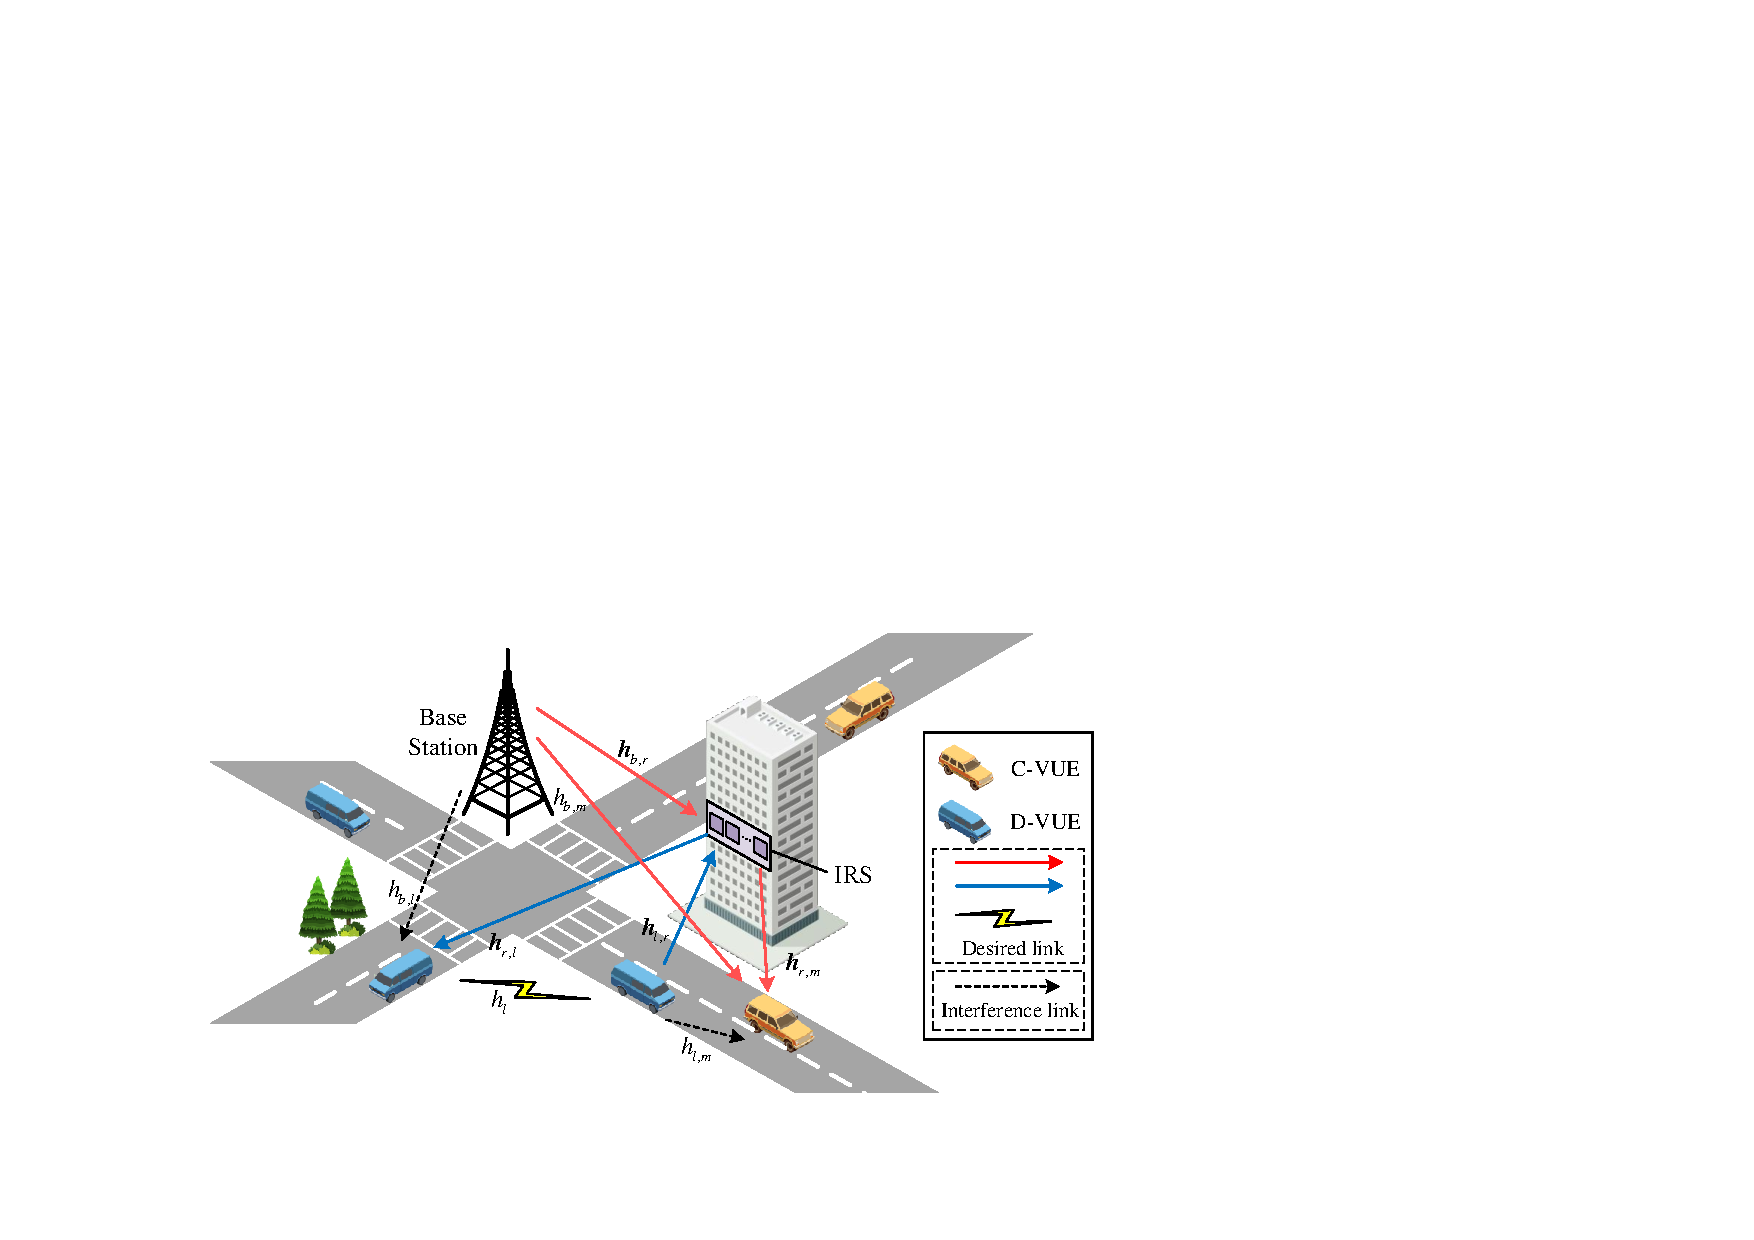
\includegraphics[width=1.0\linewidth]{Fig1.pdf}% 1\linewidth
	\caption{Intelligent reflecting surface aids vehicular communications.}  %\label{fig}
\end{figure}

Similarly, we can obtain the channel gain from the transmitter of the $l$th D2D-V2V pair to the IRS ${\bm{h}_{l,r}} \in \mathbb{C}^{{N \times 1}}$, and the channel gain from the IRS to the receiver of the $l$th D2D-V2V pair ${\bm{h}_{r,l}} \in \mathbb{C}^{{N \times 1}}$, respectively. Let ${h_l}$ denote the channel gain of the desired transmission for the $l$th D2D-V2V pair. In addition, let ${h_{b,l}}$ denote the interference channel gain from the BS to the receiver of the $l$th D2D-V2V and ${h_{l,m}}$ denote the interference channel gain from the transmitter of the $l$th D2D-V2V pair to the $m$th C-VUE.

The phase-shifts vector is defined as $\bm{\theta  = }\left[ {{\theta _1},{\theta _2},...,{\theta _N}} \right]$ and the diagonal matrix ${\bf{\Theta }} = {\rm{diag}}\left( {{\beta _1}{e^{j{\theta _1}}},{\beta _2}{e^{j{\theta _2}}},...,{\beta _N}{e^{j{\theta _N}}}} \right)$ denotes the reflection coefficients of the IRS, where ${\theta _n} \in \left[ {\left. {0,2\pi } \right)} \right.$ and ${\beta _n} \in \left[ {0,1} \right]$ represent the phase shift and amplitude reflection coefficient of the $n$th IRS reflection element, respectively. In fact, the phase shifts are usually selected from a finite number of discrete values that vary between 0 and $ 2\pi $. For simplicity of analysis, we assume that the phase shifts can be continuously varied in $ \left[ {0,2\pi } \right) $ \cite{IRS-1}. The combined channel gain from the BS to the $m$th C-VUE is ${\left| {\bm{h}_{r,m}^H{\bf{\Theta }}{\bm{h}_{b,r}} + {h_{b,m}}} \right|^2}$ and the combined channel gain of the $l$th D2D-V2V pair is ${\left| {\bm{h}_{r,l}^H{\bf{\Theta }}{\bm{h}_{l,r}} + {h_l}} \right|^2}$. Due to the high mobility of vehicles, it is difficult to track the instantaneous CSI of the mobile channel in practical applications. It is practical that the BS can use slowly varying large-scale fading \cite{IOVRM-6} \cite{IOVRM-28}. We assume that the CSI of all channels involved is perfectly known at the BS. Let $ {P_{m,k}} $ and $ {P_{l,k}} $ denote the transmit powers of the $m$th C-VUE and the transmitter of the $l$th D2D-V2V pair over the $k$th spectrum band, respectively. The binary variables ${x_{m,k}},{x_{l,k}} \in \left\{ {0,1} \right\} $ is the spectrum allocation indicator with $ {x_{m,k}}=1 $ indicating the $m$th C-VUE transmits over the $k$th spectrum band, and $ {x_{m,k}}=0 $ otherwise. The spectrum allocation indicator ${x_{l,k}}$ for the $ l $th D2D-V2V pair is similarly defined.

To this end, the received SINRs of the $m$th C-VUE and the reciever of the $l$th D2D-V2V pair can be expressed as
\begin{equation}
{\gamma _{m,k}} = \frac{{{P_{m,k}}{{\left| {\bm{h}_{r,m}^H{\bf{\Theta }}{\bm{h}_{b,r}} + {h_{b,m}}} \right|}^2}}}{{\sum\limits_{l \in {\cal L}} {{x_{l,k}}{P_{l,k}}{{\left| {\bm{h}_{r,m}^H{\bf{\Theta }}{\bm{h}_{l,r}} + {h_{l,m}}} \right|}^2}}  + {\sigma ^2}}},
\end{equation}
and
\begin{equation}
{\gamma _{l,k}} = \frac{{{P_{l,k}}{{\left| {\bm{h}_{r,l}^H{\bf{\Theta }}{\bm{h}_{l,r}} + {h_l}} \right|}^2}}}{{\sum\limits_{m \in {\cal M}} {{x_{m,k}}{P_{m,k}}{{\left| {\bm{h}_{r,l}^H{\bf{\Theta }}{\bm{h}_{b,r}} + {h_{b,l}}} \right|}^2}}  + {\sigma ^2}}},
\end{equation}
respectively, where ${\sigma ^2}$ is the noise power. Then the achievable downlink rate of the $m$th C-VUE and the achievable transmission rate of the $l$th D2D-V2V pair can be given by $ {R_m} = \sum\limits_{k \in {\cal K}} {{x_{m,k}}{{\log }_2}\left( {1 + {\gamma _{m,k}}} \right)} $ and $ {R_l} = \sum\limits_{k \in {\cal K}} {{x_{l,k}}{{\log }_2}\left( {1 + {\gamma _{l,k}}} \right)} $, respectively.
%\begin{equation}
%{R_m} = \sum\limits_{k \in {\cal K}} {{x_{m,k}}{{\log }_2}\left( {1 + {\gamma _{m,k}}} \right)} ,
%\end{equation}
%and
%\begin{equation}
%{R_l} = \sum\limits_{k \in {\cal K}} {{x_{l,k}}{{\log }_2}\left( {1 + {\gamma _{l,k}}} \right)} ,
%\end{equation}
%respectively.


To satisfy different QoS requirements for V2X links, the sum capacity of the $M$ V2I links is maximized while guaranteeing the minimum transmission SINR of the V2V links, jointly optimizing the power allocation ${\bf{P}}{\rm{ = }}\left\{ {{P_{m,k}},{P_{l,k}},\forall m,l,k} \right\}$, spectrum allocation ${\bf{X}}{\rm{ = }}\left\{ {{x_{m,k}},{x_{l,k}},\forall m,l,k} \right\}$ and the reflection-coefficient matrix $ {\bf{\Theta }} $, subject to the constraints of the IRS reflection coefficients. The problem is formulated as follows
\begin{subequations}\label{P1}
	\begin{align}
	&\mathop {\max }\limits_{\left\{ {{\bf{P}},{\bf{X}},{\bf{\Theta }}} \right\}} \quad \sum\limits_{m \in {\cal M}} {{R_m}} \\
	s.t.\qquad &{x_{m,k}},{x_{l,k}} \in \left\{ {0,1} \right\},\forall m,l,k,\\
		&\sum\limits_{m \in {\cal M}} {{x_{m,k}}}  \le 1,\sum\limits_{l \in {\cal L}} {{x_{l,k}}}  \le 1,\forall k,\\
		&\sum\limits_{k \in {\cal K}} {{x_{m,k}}}  \le 1,\sum\limits_{k \in {\cal K}} {{x_{l,k}}}  \le 1,\forall m,l,\\
	&\sum\limits_{m \in {\cal M}} {\sum\limits_{k \in {\cal K}} {{x_{m,k}}{P_{m,k}}} }  \le {P_{\max }},\nonumber\\
	&\sum\limits_{k \in {\cal K}} {{x_{l,k}}{P_{l,k}} \le P_l^{\max }} ,\forall l,\\
	&{P_{m,k}} \ge 0,{P_{l,k}} \ge 0,\forall m,l,k,\\
	&\left| {{{\bf{\Theta }}_{n,n}}} \right| \le 1,\forall n,\\
	&{\gamma _{l,k}} \ge {\gamma ^{req}},\forall l,k,
	\end{align}
\end{subequations}

\noindent where $ {\gamma ^{req}} $ is the minimum SINR needed to be satisfied for V2V links in (\ref{P1}h). (\ref{P1}c) limits orthogonal spectrum to be allocated among the V2I and V2V links. (\ref{P1}d) models our assumption that each V2I and V2V link is allocated at most one spectrum band. (\ref{P1}e) restricts that the transmission power allocated to each VUE does not exceed the maximum value, and (\ref{P1}f) ensures the non-negativity of the allocated power. (\ref{P1}g) constrains the reflection coefficients of the IRS. Due to the fact that variables ${\bf{X}}$, $ {\bf{P}} $ and ${\bf{\Theta }}$ are coupled to each other, the problem is a mix-integer non-convex problem that is rather challenging to solve. In the following sections, an effective two-stage algorithm is proposed to tackle this problem.

\section{Proposed Algorithm}
In this section, we propose a two-stage joint Resource Allocation algorithm for IRS-aided Vehicular Communications, namely RAIVC, to solve the studied problem. Since there are a total of three kinds of optimization variables in problem~(\ref{P1}), i.e., $\bf{P}$, $\bf{\Theta}$ and $\bf{X}$, it is difficult to find a globally optimal solution, so an approximate optimal algorithm is expected. In the following, we first fix the spectrum allocation variable and jointly optimize the power allocation and the IRS reflection coefficients in Stage 1. Then, based on the result of Stage~1, we try to find the optimal spectrum allcation scheme in Stage~2.

\subsection{Stage 1: Joint Optimization of Power Allocation and Reflection Coefficients}
For any given spectrum allocation $\bf{X}$, the joint optimization problem of power allocation and the IRS reflection coefficients can be formulated as
\begin{subequations}\label{P2}
	\begin{gather}
	\mathop {\max }\limits_{{\bf{P}},{\bf{\Theta }}} \quad\sum\limits_{m \in {\cal M}} {{R_m}} \\
	s.t. \qquad (\ref{P1}\rm{e})-(\ref{P1}\rm{h}).
	\end{gather}
\end{subequations}

\noindent It can be seen that the objective function is non-concave, and the slack variables $ {\bf{S}} = \left\{ {{S_{m,k}} = \frac{{{P_{m,k}}{{\left| {\bm{h}_{r,m}^H{\bf{\Theta }}{\bm{h}_{b,r}} + {h_{b,m}}} \right|}^2}}}{{\sum\nolimits_{l \in {\cal L}} {{x_{l,k}}{P_{l,k}}{{\left| {\bm{h}_{r,l}^H{\bf{\Theta }}{\bm{h}_{l,r}} + {h_{l,m}}} \right|}^2}}  + {\sigma ^2}}},\forall m,k} \right\} $ are introduced to handle the non-concavity of the objective function. Then it is satisfied that
\begin{equation}\label{*}
\small
\frac{{{P_{m,k}}{{\left| {\bm{h}_{r,m}^H{\bf{\Theta }}{\bm{h}_{b,r}} + {h_{b,m}}} \right|}^2}}}{{\sum\limits_{l \in {\cal L}} {{x_{l,k}}{P_{l,k}}{{\left| {\bm{h}_{r,l}^H{\bf{\Theta }}{\bm{h}_{l,r}} + {h_{l,m}}} \right|}^2}}  + {\sigma ^2}}} \ge {S_{m,k}},\forall m,k.
\end{equation}
Thus problem (\ref{P2}) can be equivalently transformed into
\begin{subequations}\label{P3}
	\begin{gather}
	\mathop {\max }\limits_{{\bf{P}},{\bf{\Theta }},{\bf{S}}} \quad \sum\limits_{m \in {\cal M}} {\sum\limits_{k \in {\cal K}} {{{\log }_2}\left( {1 + {S_{m,k}}} \right)} } \\
	s.t. \qquad (\ref{P1}\rm{e})-(\ref{P1}\rm{h}),(\ref{*}).
	\end{gather}
\end{subequations}

\noindent Due to the fact that the variables $ \bf{P} $ and $ \bm{\Theta} $ are coupled to each other, the non-convex problem (\ref{P3}) is still prohibitive to solve. In order to make problem (\ref{P3}) tractable, we first decompose it into the following two subproblems
\begin{subequations}\label{P3-1}
	\begin{gather}
	\mathop {\max }\limits_{{\bf{P}},{\bf{S}}} \quad \sum\limits_{m \in {\cal M}} {\sum\limits_{k \in {\cal K}} {{{\log }_2}\left( {1 + {S_{m,k}}} \right)} } \\
	s.t. \quad (\ref{P1}\rm{e}),(\ref{P1}\rm{f}),(\ref{P1}\rm{h}),(\ref{*}),
	\end{gather}
\end{subequations}
and
\begin{subequations}\label{P3-2}
	\begin{gather}
	{\rm{Find}}\quad{\bf{\Theta }}\\
	s.t. \quad (\ref{P1}\rm{g}),(\ref{P1}\rm{h}),(\ref{*}).
	\end{gather}
\end{subequations}

\noindent For given the IRS reflection coefficients, subproblem (\ref{P3-1}) focuses on finding the optimal power allocation matrix $ \bf{P} $; for fixed $ \bf{P} $, subproblem (\ref{P3-2}) focuses on finding the optimal reflection-coefficient matrix $ \bm{\Theta} $. Next, we set out to discuss how to solve the above two sub-problems.

\subsubsection{Optimization of Power Allocation}
For problem (\ref{P3-1}), the non-convex constraint (\ref{*}) needs to be dealt with according to the lemma in \cite{IRS-ARXIV-8-33}, which means that if we replace it by its convex upper bound and iteratively solve the yielding problem by judiciously updating the variables until convergence, the local optimal can be obtained. To this end, the upper bound of $ \sum\nolimits_{l \in {\cal L}} {{P_{l,k}}{S_{m,k}}} $ is given by 
\begin{equation}
	  \sum\nolimits_{l \in {\cal L}} {{P_{l,k}}{S_{m,k}}}  \le \frac{1}{2}{\alpha _{m,k}}S_{m,k}^2 + \frac{1}{{2{\alpha _{m,k}}}}{\left( {\sum\nolimits_{l \in {\cal L}} {{P_{l,k}}} } \right)^2} ,
\end{equation}
where $ {\alpha _{m,k}} = \left( {\sum\nolimits_{l \in {\cal L}} {{P_{l,k}}} } \right)/{S_{m,k}} $. The given local points $ {\alpha _{m,k}} $ can be updated in the $r$th iteration according to $ \alpha _{m,k}^{\left( r \right)} = \left( {\sum\nolimits_{l \in {\cal L}} {P_{l,k}^{\left( {r - 1} \right)}} } \right)/S_{m,k}^{\left( {r - 1} \right)} $, and the constraint (\ref{*}) can be rewritten as
\begin{equation}\label{triangle}
\small
\setlength\abovedisplayskip{1pt}
\setlength\belowdisplayskip{1pt}
	{P_{m,k}}A \ge \frac{1}{2}\alpha _{m,k}^{\left( r \right)}S_{m,k}^2{\rm{ + }}\frac{1}{{2\alpha _{m,k}^{\left( r \right)}}}{\left( {\sum\limits_{l \in {\cal L}} {{x_{l,k}}{P_{l,k}}} B} \right)^2} + {S_{m,k}}{\sigma ^2},\forall m,k,
\end{equation}
where $ A = {\left| {\bm{h}_{r,m}^H{\bf{\Theta }}{\bm{h}_{b,r}} + {h_{b,m}}} \right|^2} $ and $ B = {\left| {\bm{h}_{r,l}^H{\bf{\Theta }}{\bm{h}_{l,r}} + {h_{l,m}}} \right|^2}$. Then problem
(\ref{P3-1}) is approximated as the following problem
\begin{subequations}\label{P4}
	\begin{gather}
	\mathop {\max }\limits_{{\bf{P}},{\bf{S}}} {\rm{    }}\sum\limits_{m \in {\cal M}} {\sum\limits_{k \in {\cal K}} {{{\log }_2}\left( {1 + {S_{m,k}}} \right)} } \\
	s.t. \quad (\ref{P1}\rm{e}),(\ref{P1}\rm{f}),(\ref{P1}\rm{h}),(\ref{triangle}).
	\end{gather}
\end{subequations}

\noindent Problem (\ref{P4}) is a convex optimization problem, and the optimal solution can be effectively obtained by the convex optimization solving tools such as CVX \cite{book-Convex}.

%\textit{Remark 1:} In each iteration, for given random initial points $ {{\bf{P}}^{\left( 0 \right)}} $ and $ {{\bf{S}}^{\left( 0 \right)}} $, problem (\ref{P4}) may not be feasible. Feasible initial points are  essential if feasible solutions can be obtained. In general, finding feasible points is difficult. Next we formulate a feasibility problem and propose a novel feasible point search algorithm. The formulated problem is $ {l_1} - \min $ problem, which can be given by in the $ v $th iteration


\subsubsection{Design of the IRS Reflection Coefficients}
The combined channel gain $ {\left| {\bm{h}_{r,m}^H{\bf{\Theta }}{\bm{h}_{b,r}} + {h_{b,m}}} \right|^2} $ can be rewritten as
\begin{equation}
{\left| {\bm{h}_{r,m}^H{\bf{\Theta }}{\bm{h}_{b,r}} + {h_{b,m}}} \right|^2} = {\left| {\bm{z}{\bf{\Phi }} + {h_{b,m}}} \right|^2},
\end{equation}
where $ \bm{z} = \bm{h}_{r,m}^H{\rm{diag}}\left\{ {{\bm{h}_{b,r}}} \right\} $ and $ {\bf{\Phi }} = {\left( {{\beta _1}{e^{j{\theta _1}}},...,{\beta _N}{e^{j{\theta _N}}}} \right)^T} $. Slack variables $ \bm{\kappa  = }\left\{ {{\kappa _m} = {\mathop{\rm Re}\nolimits} \left( {\bm{z}{\bf{\Phi }} + {h_{b,m}}} \right),\forall m} \right\} $ and $\bm{\xi  = }\left\{ {{\xi _m} = {\mathop{\rm Im}\nolimits} \left( {\bm{z}{\bf{\Phi }} + {h_{b,m}}} \right),\forall m} \right\}$ are introduced, where $ \kappa _m^2 + \xi _m^2$$={\left| {z{\bf{\Phi }} + {h_{b,m}}} \right|^2}$. Similarly, for the combined channel gain $ {\left| {\bm{h}_{r,l}^H{\bf{\Theta }}{\bm{h}_{l,r}} + {h_{l,m}}} \right|^2} $, slack variables $\bm{\eta } = \left\{ {{\eta _l} = } \right.{\mathop{\rm Re}\nolimits} \left( {\tilde{\bm{z}}{\bf{\Phi }} + } \right.$\\ $\left. {\left. {{h_{l,m}}} \right),\forall l} \right\}$ and $\bm{\omega  = }\left\{ {{\omega _l} = {\mathop{\rm Im}\nolimits} \left( {\tilde{\bm{z}}{\bf{\Phi }} + {h_{l,m}}} \right),\forall l} \right\}$ are introduced, where $ \tilde{\bm{z}} = \bm{h}_{r,l}^H{\rm{diag}}\left( {{\bm{h}_{l,r}}} \right) $. Meanwhile, it should be satisfied that $ \eta _l^2 + \omega _l^2 = {\left| {\tilde{\bm{z}}{\bf{\Phi }} + {h_{l,m}}} \right|^2} $. To this end, problem~(\ref{P3-2}) can be reformulated as a feasibility-check problem as follows
\begin{subequations}\label{P6}
	\begin{gather}
	{\rm{Find}}\quad{\bf{\Phi }}\\
	s.t.\quad \left| {{\Phi _n}} \right| \le 1,\forall n,\\
		{\kappa _m} = {\mathop{\rm Re}\nolimits} \left( {\bm{z}{\bf{\Phi }} + {h_{b,m}}} \right),{\xi _m} = {\mathop{\rm Im}\nolimits} \left( {\bm{z}{\bf{\Phi }} + {h_{b,m}}} \right),\forall m,\\
		{\eta _l} = {\mathop{\rm Re}\nolimits} \left( {\tilde{\bm{z}}{\bf{\Phi }} + {h_{l,m}}} \right),{\omega _l} = {\mathop{\rm Im}\nolimits} \left( {\tilde{\bm{z}}{\bf{\Phi }} + {h_{l,m}}} \right),\forall l,\\
	\frac{{{P_{m,k}}\left( {\kappa _m^2 + \xi _m^2} \right)}}{{\sum\limits_{l \in {\cal L}} {{x_{l,k}}{P_{l,k}}\left( {\eta _l^2 + \omega _l^2} \right)}  + {\sigma ^2}}} \ge {S_{m,k}},\forall m,k.
	\end{gather}
\end{subequations}


To tackle the non-convexity of (\ref{P6}e), the successive convex approximation technique can be applied in each iteration. With given local points $ \left( {\kappa _{m,k}^{\left( r \right)},\xi _{m,k}^{\left( r \right)}} \right) $, the lower bound of $ \kappa _m^2 + \xi _m^2 $, denoted by $ \Gamma _m^{lb} $, can be found according to the first-order Taylor expansion~\cite{book-Convex}, which follows 
\begin{align}
	 \kappa _m^2 + \xi _m^2 &\ge {\left( {\kappa _m^{\left( r \right)}} \right)^2} + {\left( {\xi _m^{\left( r \right)}} \right)^2} \\
	 &+ 2\kappa _m^{\left( r \right)}\left( {{\kappa _m} - \kappa _m^{\left( r \right)}} \right) + 2\xi _m^{\left( r \right)}\left( {{\xi _m} - \xi _m^{\left( r \right)}} \right)\\
	 &= \Gamma _m^{lb} ,
\end{align} 
Therefore, problem (\ref{P6}) can be further formulated as
\begin{subequations}\label{P7}
	\begin{gather}
	{\rm{Find}}\quad{\bf{\Phi }}\\
	s.t. \quad \frac{{{P_{m,k}}\Gamma _m^{lb}}}{{\sum\limits_{l \in {\cal L}} {x_{l,k}^{\left( t \right)}{P_{l,k}}\left( {\eta _l^2 + \omega _l^2} \right)}  + {\sigma ^2}}} \ge {S_{m,k}},\forall m,k,\\
	(\ref{P6}\rm{b})-(\ref{P6}\rm{d}).
	\end{gather}
\end{subequations}

\noindent Problem (\ref{P7}) is a convex optimization problem, and can be solved effectively by using CVX.


\subsection{Stage 2: Optimization of Spectrum Allocation}
For any given power allocation $ \bf{P} $ and the IRS reflection coefficients $ \bf{\Theta} $, the spectrum allocation of problem (\ref{P1}) can be optimized by solving the following problem
\begin{subequations}\label{P8}
	\begin{gather}
	\mathop {\min }\limits_{\bf{X}}\quad-\sum\limits_{m \in {\cal M}} {\sum\limits_{k \in {\cal K}} {{x_{m,k}}{{\log }_2}\left( {1 + {\gamma _{m,k}}} \right)} } \\
	s.t.\quad (\ref{P1}\rm{b})-(\ref{P1}\rm{e}),(\ref{P1}h).
	\end{gather}
\end{subequations}

\noindent Due to the the non-convexity of the objective function and binary variables $ \bf{X} $, problem (\ref{P8}) is a mixed integer non-convex problem. To make problem (\ref{P8}) more tractable, we first relax the binary variables in (\ref{P1}b) into continuous variables. Auxiliary slack variables $ \bm{\varphi}  = \left\{ {{\varphi _{m,k}} = {{\log }_2}\left( {1 + {\gamma _{m,k}}} \right),\forall m,k} \right\} $ are introduced, which leads to the bilinear part $ {{x_{m,k}}{\varphi _{m,k}}} $. Meanwhile, the constraint $ {\varphi _{m,k}} \le {\log _2}\left( {1 + {\gamma _{m,k}}} \right) $ should be satisfied. To deal with these non-convex factors, $ - {x_{m,k}}{\varphi _{m,k}}$ can be written as the difference between two convex functions, which is given by
%\begin{subequations}\label{P9}
%	\begin{align}
%	&\mathop {\min }\limits_{{\bf{X}},\varphi } \quad - \sum\limits_{m \in {\cal M}} {\sum\limits_{k \in {\cal K}} {{x_{m,k}}{\varphi _{m,k}}} } \\
%	s.t.\quad &{x_{m,k}},{x_{l,k}} \in \left[ {0,1} \right],\forall m,l,k,\\
%	&{\varphi _{m,k}} \le {\log _2}\left( {1 + {\gamma _{m,k}}} \right),\forall m,k,\\
%	&(\ref{P1}\rm{b})-(\ref{P1}\rm{e}),(\ref{P1}h).
%	\end{align}
%\end{subequations}
\begin{small}
\setlength\abovedisplayskip{2pt}
\setlength\belowdisplayskip{3pt}
	\begin{subequations}
		\begin{align}
		&- {x_{m,k}}{\varphi _{m,k}} = \frac{1}{2}x_{m,k}^2 + \frac{1}{2}\varphi _{m,k}^2 - \frac{1}{2}{\left( {{x_{m,k}} + {\varphi _{m,k}}} \right)^2}\nonumber\\
		&\mathop  \le \limits^{\left( a \right)} \frac{1}{2}x_{m,k}^2 + \frac{1}{2}\varphi _{m,k}^2 - \frac{1}{2}{\left( {x_{m,k}^{\left( r \right)} + \varphi _{m,k}^{\left( r \right)}} \right)^2}\nonumber\\
		&- \left( {x_{m,k}^{\left( r \right)} + \varphi _{m,k}^{\left( r \right)}} \right)\left( {{x_{m,k}} - x_{m,k}^{\left( r \right)}} \right) - \left( {x_{m,k}^{\left( r \right)} + \varphi _{m,k}^{\left( r \right)}} \right)\left( {{\varphi _{m,k}} - \varphi _{m,k}^{\left( r \right)}} \right)\nonumber\\
		&= \Lambda _{m,k}^{ub},
		\end{align}
	\end{subequations}
\end{small}
where (a) holds since any concave function is globally upper-bounded by its first-order Taylor expansion at any point \cite{book-Convex} with given points $x_{m,k}^{\left( r \right)} $ and $ \varphi _{m,k}^{\left( r \right)} $ in the $r$th iteration. Similarly, the convex function $ {\log _2}\left( {1 + {\gamma _{m,k}}} \right) $ can be lower-bounded by its first-order Taylor expansion with given points $ x_{l,k}^{\left( r \right)} $, which follows 
\begin{align}
	{\log _2}\left( {1 + {\gamma _{m,k}}} \right) &\ge {\log _2}\left( {1 + \gamma _{m,k}^{\left( r \right)}} \right) + {\Delta _{m,k}}\sum\limits_{l \in {\cal L}} {\left( {{x_{l,k}} - x_{l,k}^{\left( r \right)}} \right)}  \nonumber\\
	&= R_{m,k}^{lb} ,
\end{align}
$\scriptstyle {\Delta _{m,k}} $ is the coefficient related to the derivative that is not dominant and omitted here. Thus, problem (\ref{P8}) is further transformed into the following problem
\begin{subequations}\label{P10}
	\begin{align}
	&\mathop {\min }\limits_{{\bf{X}},\bm{\varphi} } \quad \sum\limits_{m \in {\cal M}} {\sum\limits_{k \in {\cal K}} {\Lambda _{m,k}^{ub}} } \\
	s.t.\quad &{x_{m,k}},{x_{l,k}} \in \left[ {0,1} \right],\forall m,l,k,\\
    &{\varphi _{m,k}} \le R_{m,k}^{lb},\forall m,k,\\
	&(\ref{P1}\rm{c})-(\ref{P1}\rm{e}),(\ref{P1}h).
	\end{align}
\end{subequations}

\noindent Note that problem (\ref{P10}) is a convex optimization problem, and the optimal solution can be effectively obtained by the convex
optimization solving tools such as CVX.


\textit{Remark 1:} It is noted that the spectrum variables $ \bf{X} $ obtained from problem (\ref{P10}) are continuous values between 0 and 1, which means that the binary variables of the spectrum allocation needs to be reconstructed. The rule of reconstruction is to maximize the objective function of problem (\ref{P1}), i.e., $ {m^*} = \arg \mathop {\max }\limits_m \frac{{\partial \left( {\sum\nolimits_{m \in {\cal M}} {{R_m}} } \right)}}{{\partial {x_{m,k}}}} $ and $ {l^*} = \arg \mathop {\max }\limits_l \frac{{\partial \left( {\sum\nolimits_{m \in {\cal M}} {{R_m}} } \right)}}{{\partial {x_{l,k}}}} $, where $ x_{{m^*},k}^* = 1 $ and $ x_{{l^*},k}^* = 1$ indicate the suboptimal spectrum allocation variables, respectively.



%\begin{figure*}[!htb]
%	\centering
%	\subfigure[Sum V2I capacity versus the number of reflecting elements.]{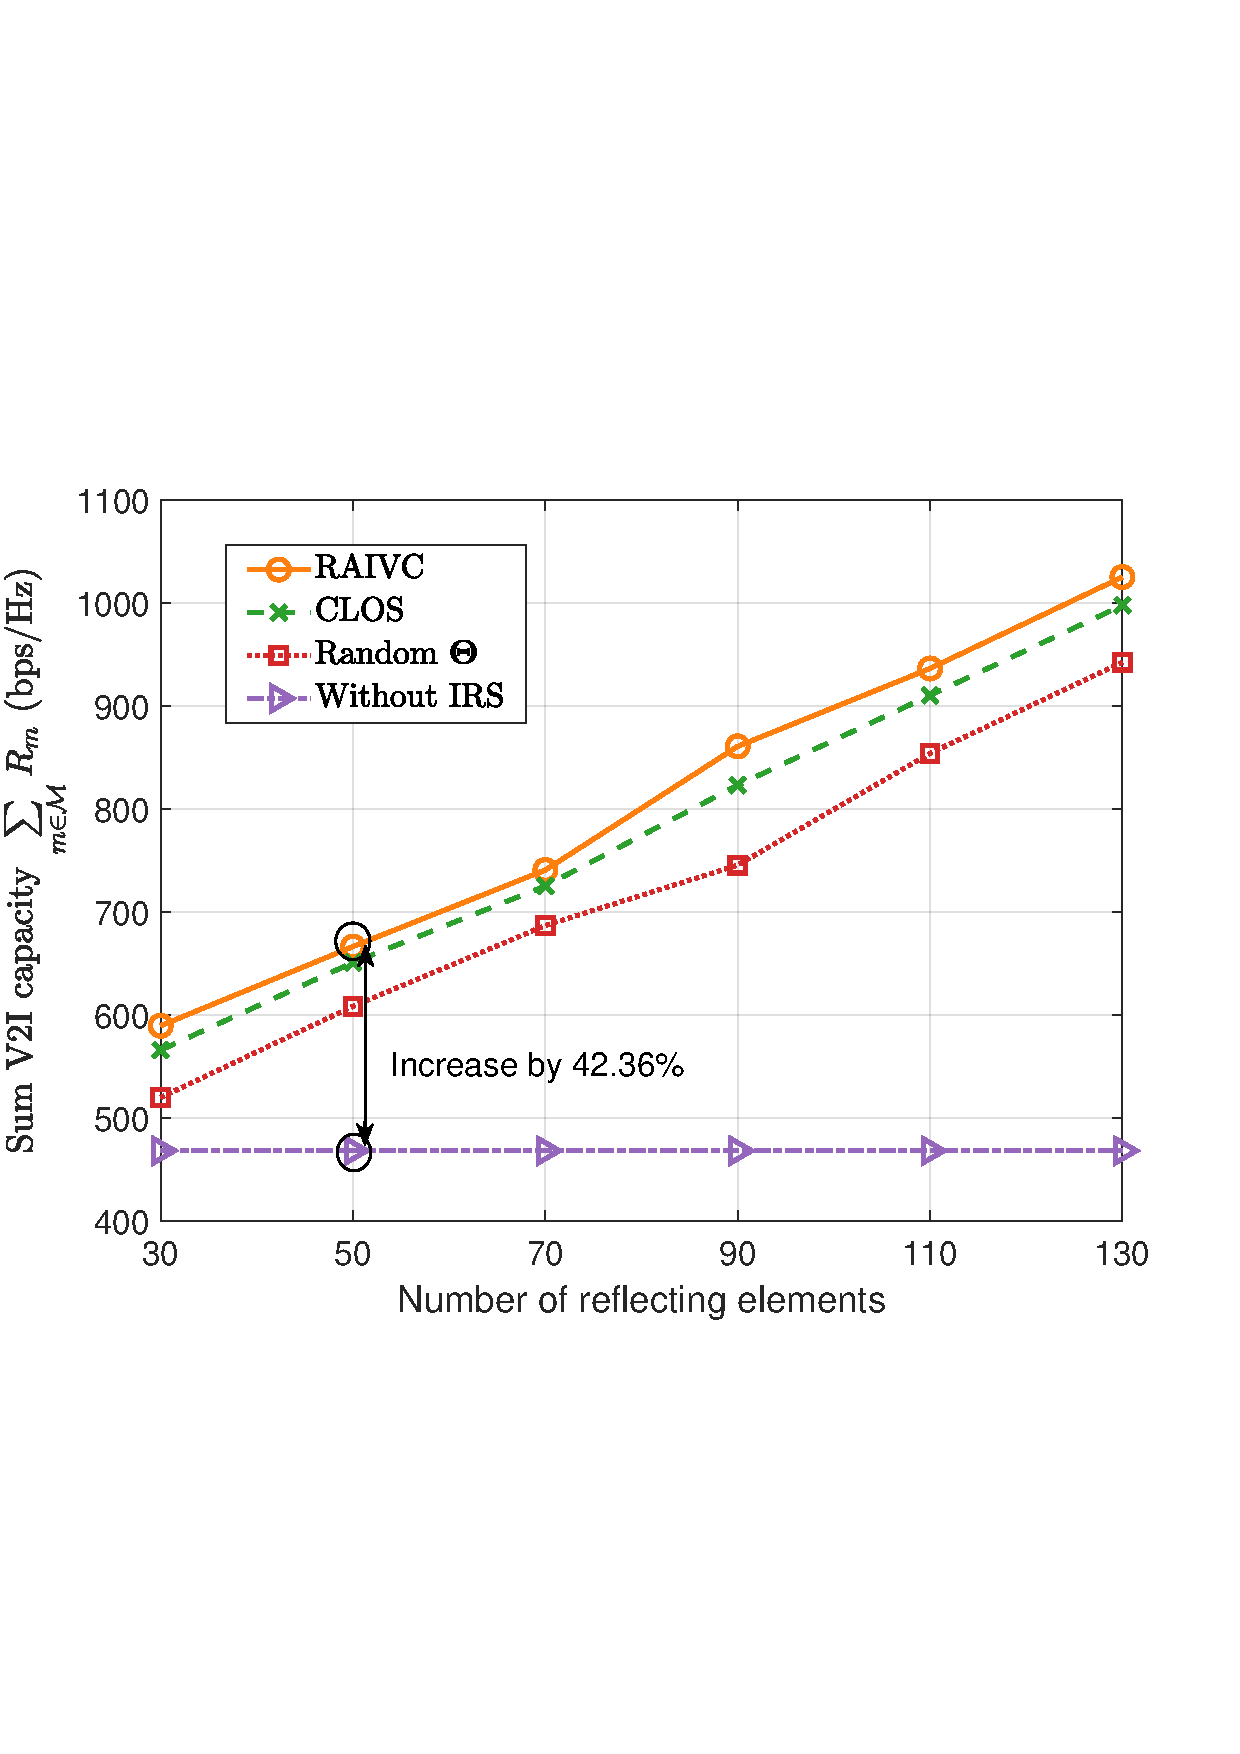
\includegraphics[width=0.3\textwidth]{Fig3.pdf}}
%	\subfigure[Sum V2I capacity versus the location of the IRS coordinate.]{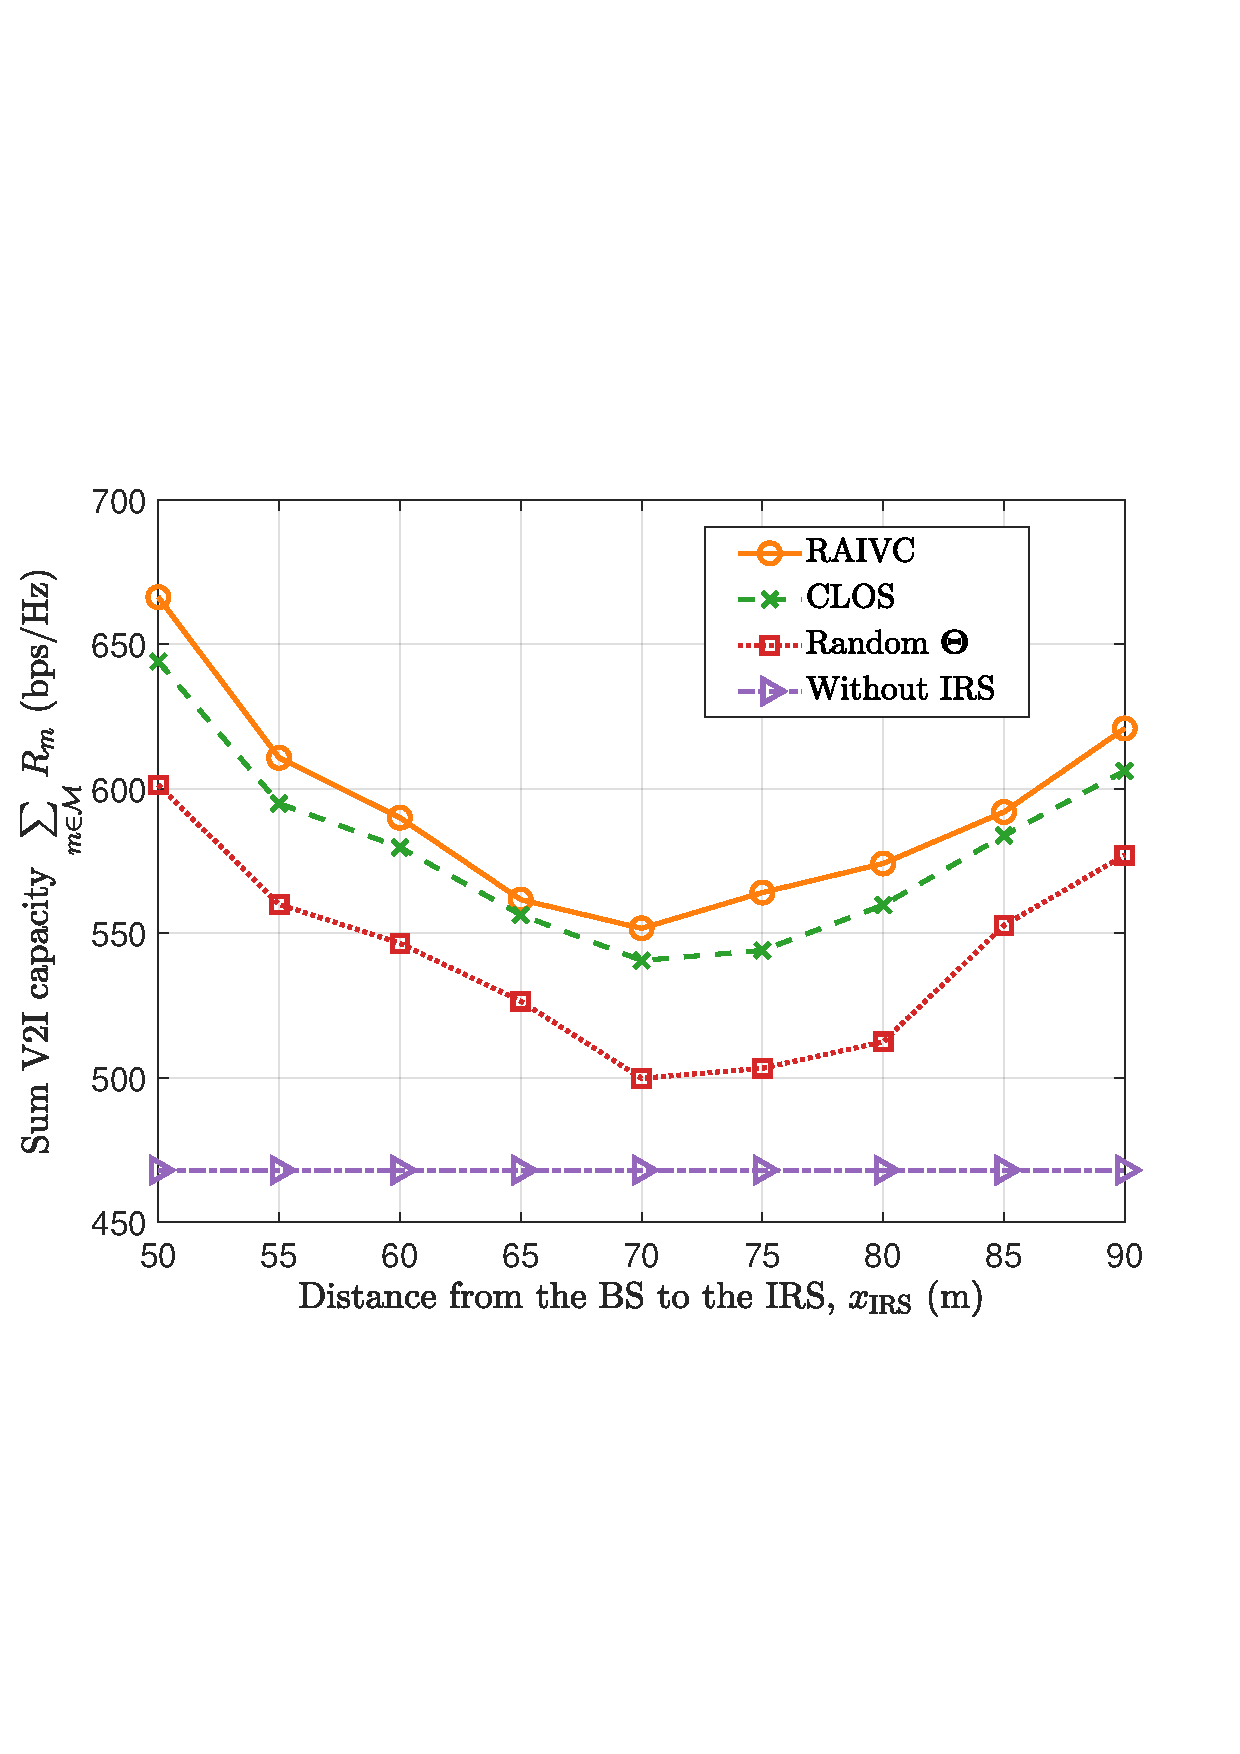
\includegraphics[width=0.3\textwidth]{Fig4.pdf}}
%	\subfigure[Sum V2I capacity versus varying vehicle speed.]{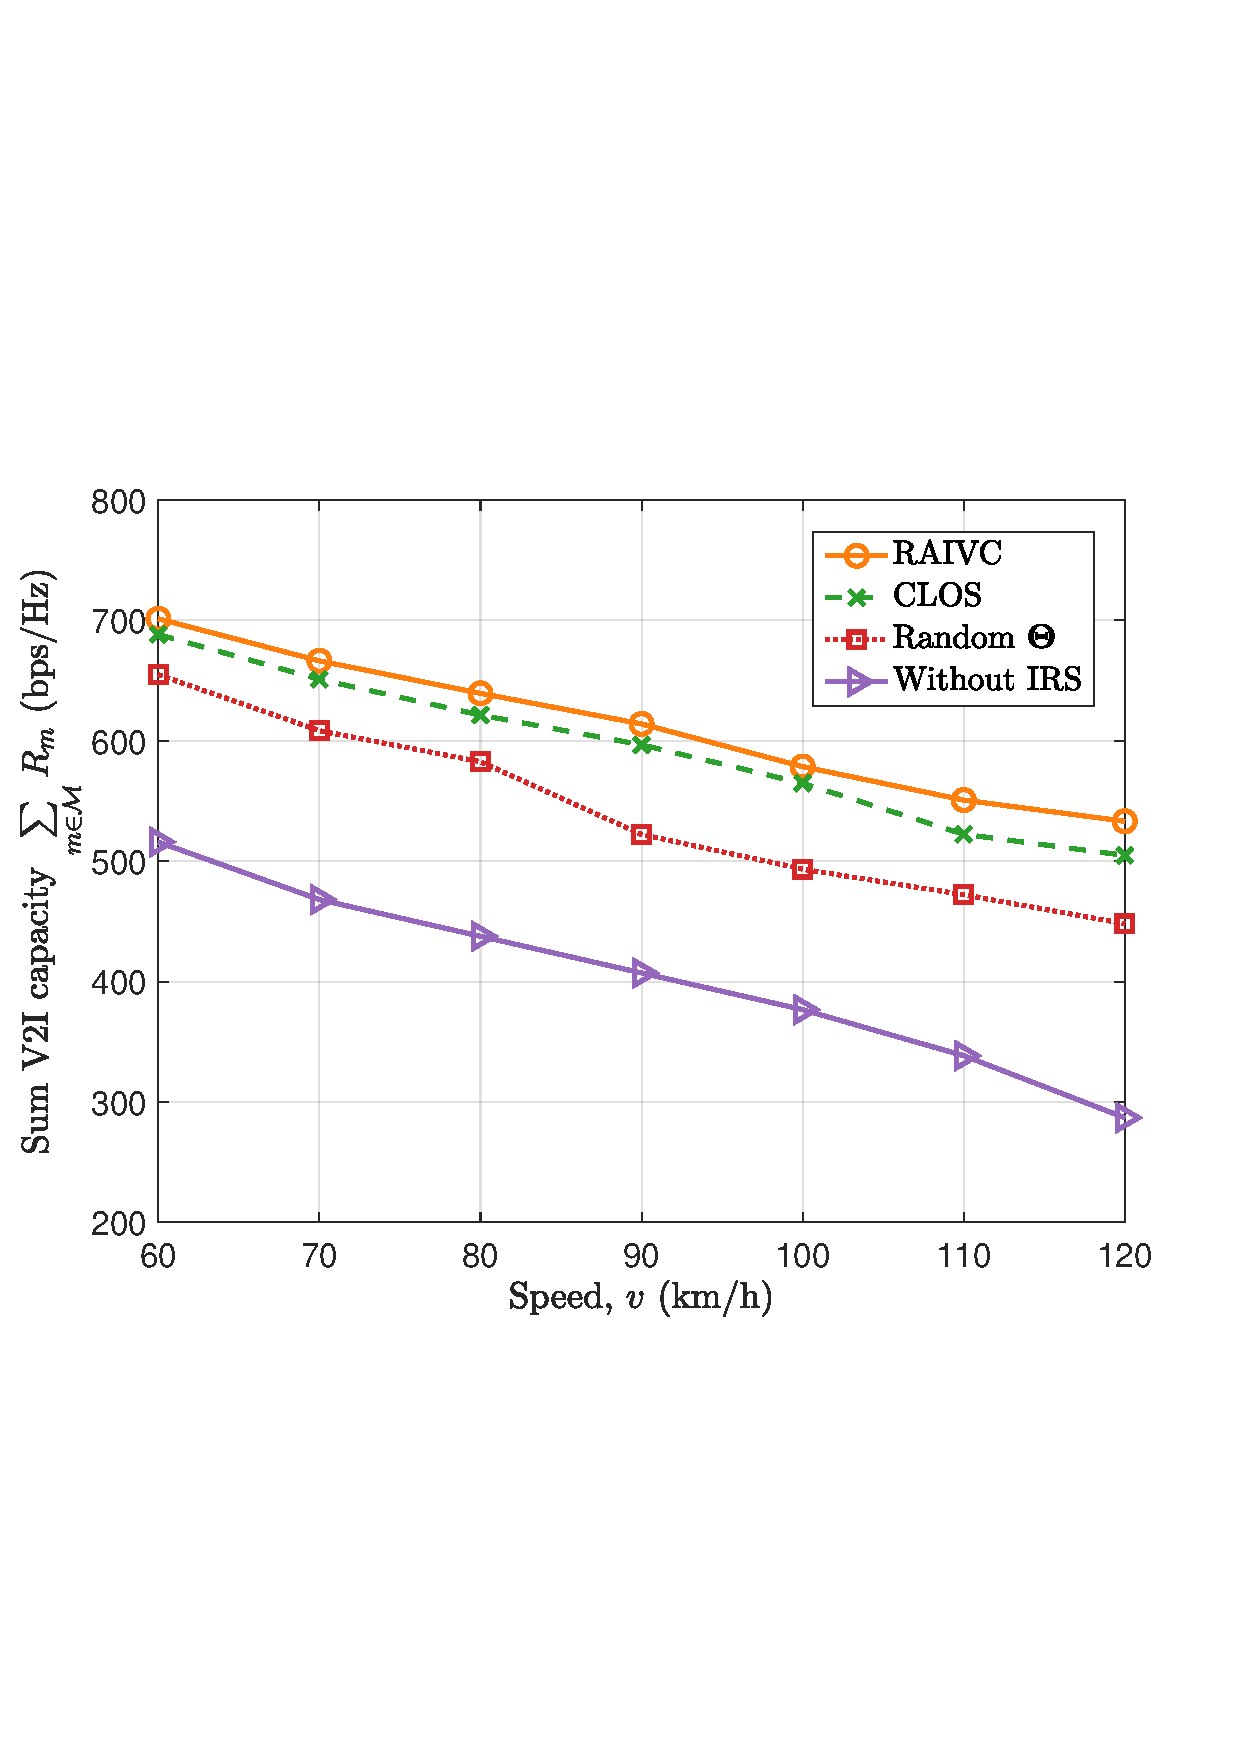
\includegraphics[width=0.3\textwidth]{Fig5.pdf}} 
%	\caption{Impact of different parameters on the sum V2I capacity.}
%	\label{Fig}
%	%	\vspace{0.2in}
%\end{figure*}


\subsection{RAIVC Algorithm}
Based on the results presented in the previous two subsections, we propose a two-stage alternating iterative algorithm called RAIVC for problem~(\ref{P1}). Specifically, in the $(r+1)$th iteration, the optimal power allocation and IRS reflection coefficients can be achieved in Stage 1 based on fixed $ \left\{ {{{\bf{X}}^{\left( r \right)}}} \right\} $, yielding the sum V2I capacity $  \sum\nolimits_{m \in {\cal M}} {{R_m}\left( {{{\bf{P}}^{\left( {r + 1} \right)}},{{\bf{\Theta}} ^{\left( {r + 1} \right)}},{{\bf{X}}^{\left( r \right)}}} \right)}  $. Then, relying on given $ \left\{ {{{\bf{P}}^{\left( {r + 1} \right)}},{{\bf{\Theta }}^{\left( {r + 1} \right)}}} \right\} $, in Stage 2, we obtain the optimal spectrum allocation $ {{{\bf{X}}^{\left( r+1 \right)}}} $ and the pseudo-optimal sum V2I capacity $ \sum\nolimits_{m \in {\cal M}} {{R_m}\left( {{{\bf{P}}^{\left( {r + 1} \right)}},{{\bf{\Theta}} ^{\left( {r + 1} \right)}},{{\bf{X}}^{\left( r+1 \right)}}} \right)}  $ in the $(r+1)$th iteration of the proposed RAIVC. The overall algorithm stops iterating when $ \sum\nolimits_{m \in {\cal M}} {\left( {R_m^{\left( {r + 1} \right)} - R_m^{\left( r \right)}} \right)} /R_m^{\left( {r + 1} \right)} \le \varepsilon $ is satisfied. The procedure of the RAIVC is summarized in Algorithm 1.

The complexity of the proposed RAIVC algorithm mainly stems from Step 3 and Step 4. To be specific, in Step 3, the complexities of solving problem (\ref{P4}) and (\ref{P7}) with the interior-point method are both $ {\cal O}\left( {{{\left( {MLK} \right)}^{3.5}}} \right) $ \cite{chen}. In Step 4, similarly, solving convex problem (\ref{P10}) with the interior-point method results in the complexity of $ {\cal O}\left( {{{\left( {MLK} \right)}^{3.5}}} \right) $. Let $ {r_{\max }} $ denote the maximum number of iterations that allows RAIVC to converge. Thus, the complexity of the proposed RAIVC algorithm can be given by $ {\cal O}\left( {{r_{\max }}{{\left( {MLK} \right)}^{3.5}}} \right)$. 

\begin{algorithm}[t]
	\caption{Two-Stage Joint \textbf{R}esource \textbf{A}llocation Algorithm for \textbf{I}RS-aided \textbf{V}ehicular \textbf{C}ommunications (RAIVC)}
	\begin{algorithmic}[1]
		\STATE {Initialize ${{\bf{P}}^{\left( 0 \right)}}$ and ${{\bf{S}}^{\left( 0 \right)}}$. Set the iterative number $v = 0$.}
		\REPEAT
		\STATE {\textbf{Stage 1:} For fixed $ \left\{ {{{\bf{X}}^{\left( r \right)}}} \right\} $, solve problem (\ref{P4}) for given $ \left\{ {{{\bf{\Theta }}^{\left( r \right)}}} \right\} $ and solve the feasibility-check problem~(\ref{P7}) for given $\left\{ {{{\bf{P}}^{\left( r \right)}}} \right\}$. Denote the optimal solution as $\left\{ {{{\bf{P}}^{\left( {r + 1} \right)}},{{\bf{\Theta }}^{\left( {r + 1} \right)}}} \right\}$.} 
		\STATE {\textbf{Stage 2:} Solve problem (\ref{P10}) for given $\left\{ {{{\bf{P}}^{\left( {r + 1} \right)}},} \right.$ $\left. {{{\bf{\Theta }}^{\left( {r + 1} \right)}}} \right\}$, and denote the optimal solution as $\left\{ {{{\bf{X}}^{\left( {r + 1} \right)}}} \right\}$.}
		\STATE {Update $r = r+1 $.}
		\UNTIL {The change of the objective value is below a threshold $\varepsilon > 0$.}
	\end{algorithmic}
\end{algorithm}

\section{Simulation Results}
In this section, simulation results are presented to verify the proposed RAIVC algorithm for IRS-aided vehicular networks. The simulated setup for the highway case detailed in 3GPP TR 36.885 is follwed, where a multi-lane freeway passes through a single cell with the BS at the center of the cell~\cite{3GPP}~\cite{Simulation}. We model a total of six lanes where there exist three lanes with $4\  \rm{m}$ width in each direction. The vehicles are dropped on the roads according to spatial Poisson process and the vehicle density depends on  the vehicle speed, where the average distance between vehicles is $2.5v$ ($v$ in m/s). The absolute vehicle speed is set to $v=70\ \rm{km/h}$. The three-dimensional coordinates of the BS and IRS are $ \left( {0,0,25\ {\rm{m}}} \right) $ and $ \left( {50\ {\rm{m}},0,25\ {\rm{m}}} \right) $, respectively. The path loss exponents for BS-VUEs link, BS-IRS
link and IRS-VUEs link are 3, 2.2 and 2.5, respectively. The Rician factor is configured as $3\ \rm{dB}$. Other related system parameters are set as follows: $ {\sigma ^2} =  - 114 \ {\rm{dBm}} $, $ \rho  =  - 20\ {\rm{dB}} $, ${\gamma ^{req}} = 5\ {\rm{dB}}$, $ {P_{\max }} = P_l^{\max } = 23\ {\rm{dBm}} $, $M = L = 10$, and $N=50$.


Figure \ref{Fig3} plots the sum V2I capacity versus the number of IRS reflecting elements. We set three other benchmark schemes: 1) CLOS: \textbf{C}ombine the \textbf{L}ocal \textbf{O}ptimal \textbf{S}olutions of the Satge 1 and Stage 2 into a global solution of the original problem; 2) Random $ \bm{\Theta} $: the elements in IRS reflection-coefficient matrix are randomly set to $ {{\bf{\Theta }}_{n,n}} \in \left( {0,1} \right] $; 3) Without IRS: vehicular communications without IRS. It should be noted that the iteration is not considered in the scheme CLOS, which implies that the solutions obtained by the scheme CLOS are not globally optimal. To illustrate the effectiveness and accuracy of the RAIVC based on alternating iteration to solve problem (\ref{P1}), we use CLOS as one of the benchmark schemes. As shown in Fig.~\ref{Fig3}, the sum V2I capacity achieved by the RAIVC algorithm is significantly larger than that of other algorithms. The sum V2I capacity tends to increase significantly with the increment of the number of IRS reflecting elements. This is because more IRS passive reflecting elements are able to reflect more power of the signal received from the BS, which results in more power gain. For example, when $N = 50$, compared to the scheme without IRS, the sum of V2I capacity for the RAIVC algorithm is increased by 42.36\%. 

\begin{figure}[t]
	%	Requires \usepackage{graphicx}
	\centering
	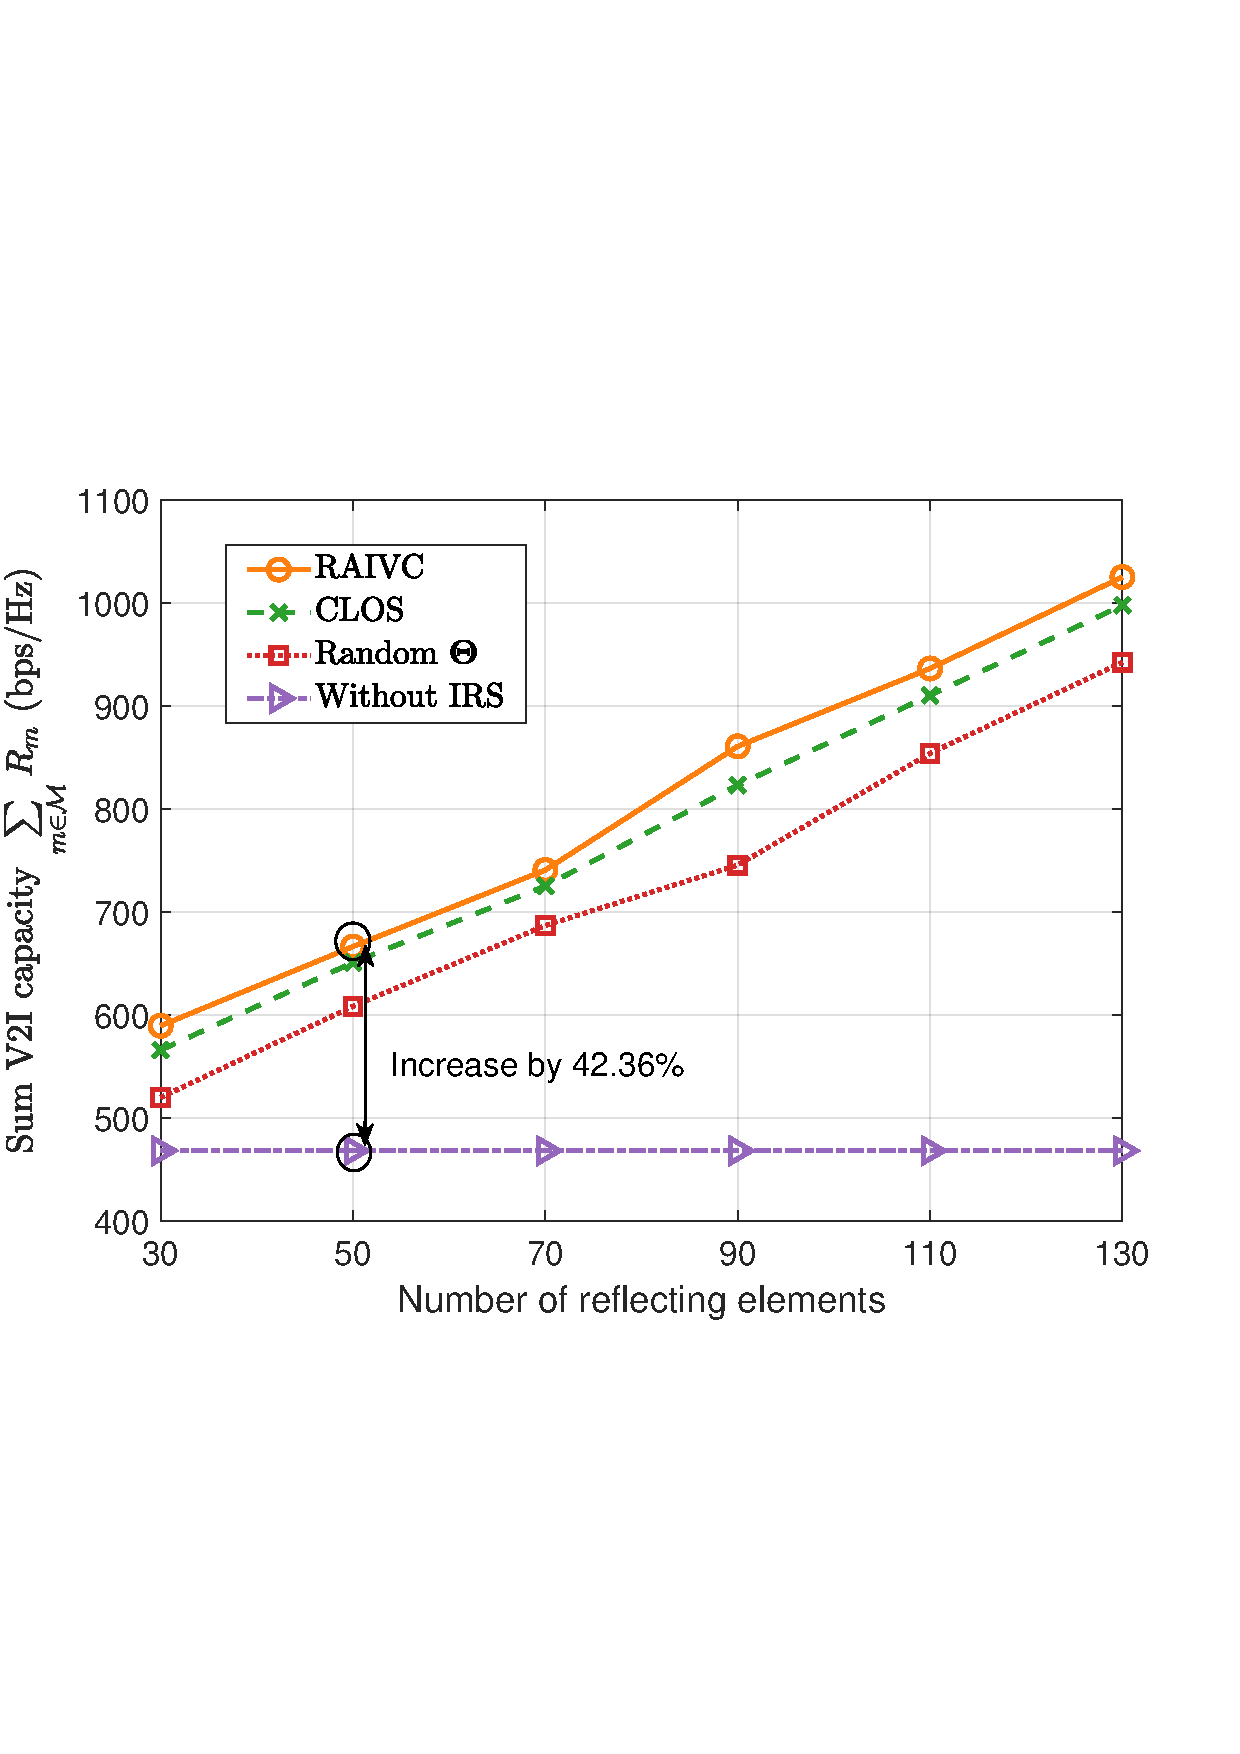
\includegraphics[width=0.8\linewidth]{Fig3.pdf}% 1\linewidth
	\caption{Sum V2I capacity versus the number of reflecting elements.}\label{Fig3}
\end{figure}

\begin{figure}[t]
	%	Requires \usepackage{graphicx}
	\centering
	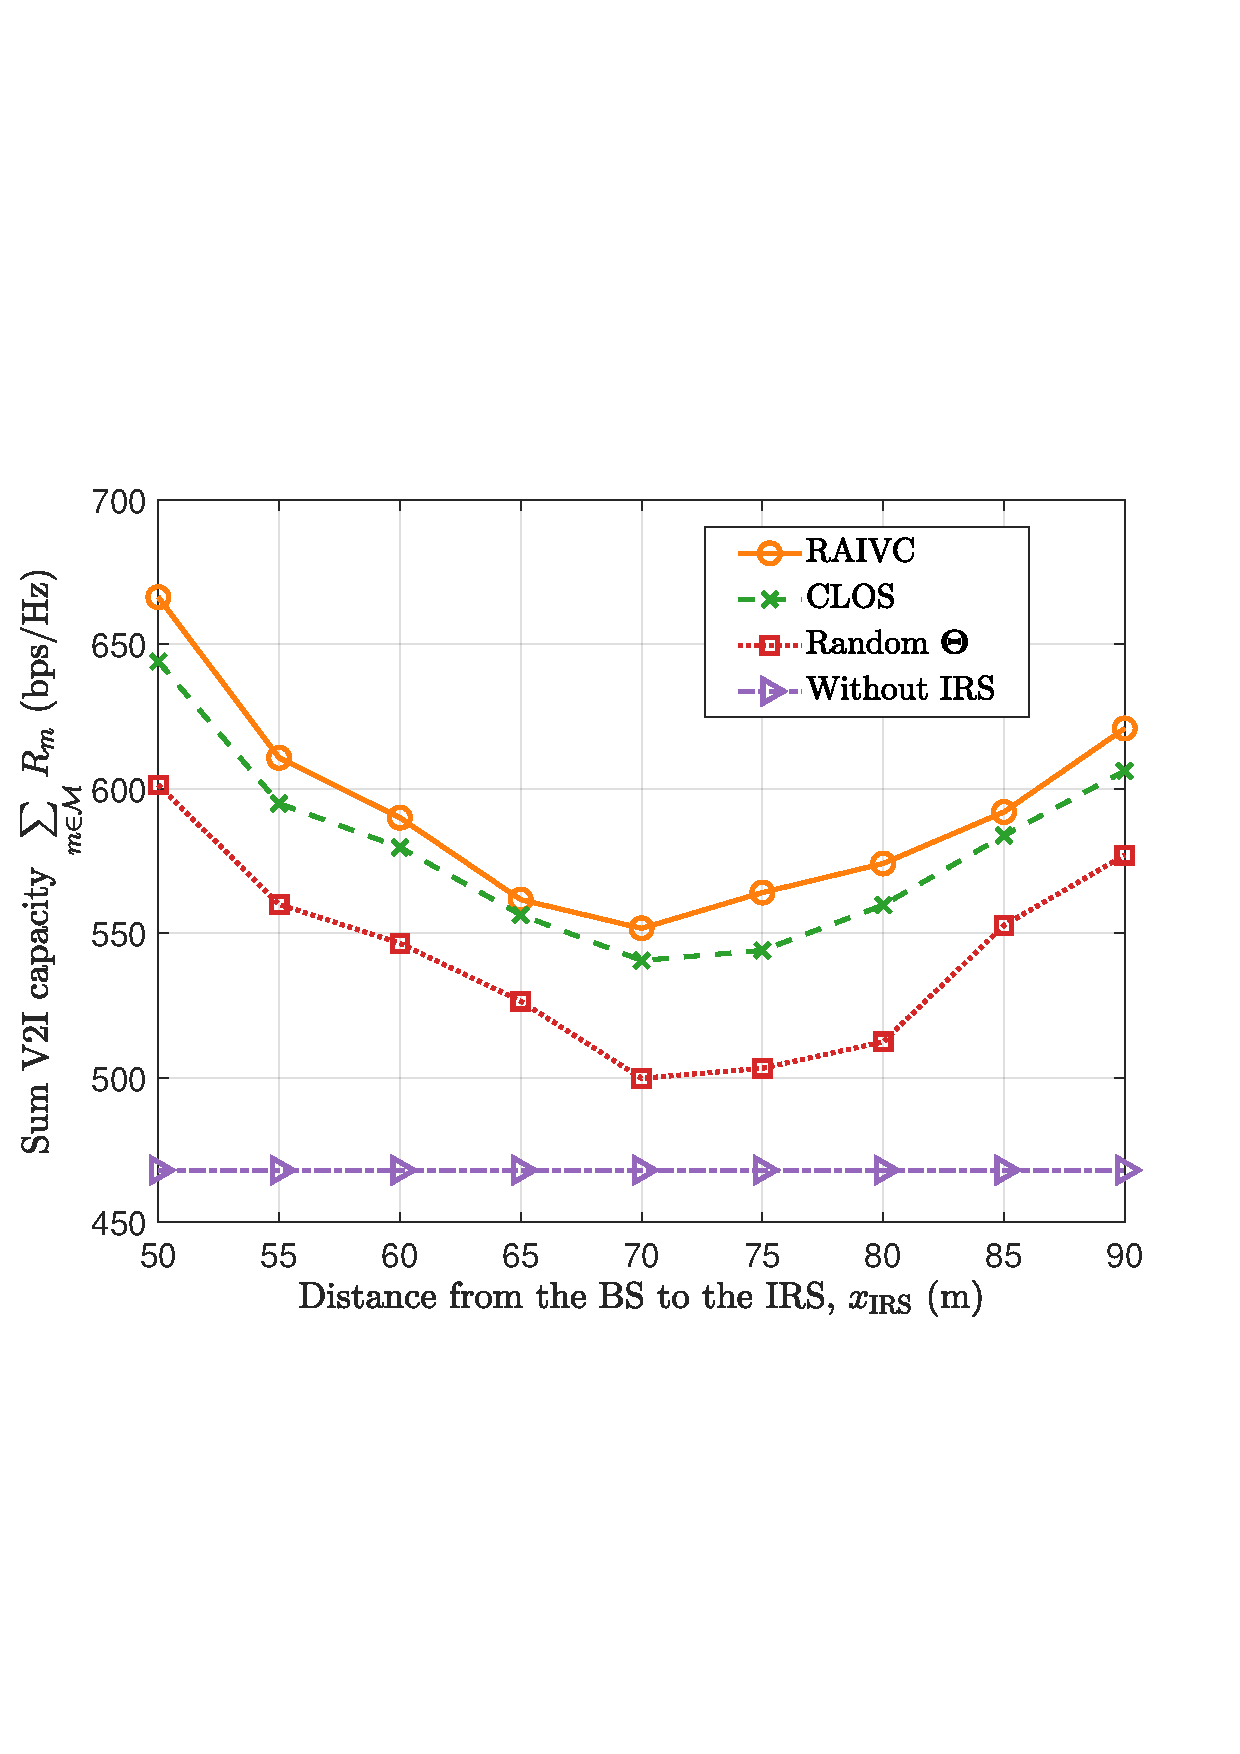
\includegraphics[width=0.8\linewidth]{Fig4.pdf}% 1\linewidth
	\caption{Sum V2I capacity versus the location of the IRS coordinate.}\label{Fig4}
\end{figure}

The impact of the IRS location on the sum V2I capacity is demonstrated in Fig. \ref{Fig4}. The coordinates of the BS and IRS are set to $ \left( {0,0,25\ {\rm{m}}} \right) $ and $ \left( {{x_{{\rm{IRS}}}},0,25\ {\rm{m}}} \right) $, respectively, that is, the distance from the BS to the IRS is $ {{x_{{\rm{IRS}}}}\rm{(m)}} $. It can be observed that RAIVC outperforms three other schemes in terms of the sum of V2I capacity. As $ {x_{{\rm{IRS}}}} $ increases, the sum V2I capacity first decreases and then increases after achieving the minimum at $ {x_{{\rm{IRS}}}} = 70{\rm{m}} $, which illustrates that the deployment of IRS will affect the actual communication effect. The reasons for this phenomenon can be attributed to the following facts. Since the vehicles are dropped according to the spatial Poisson process in our simulation, the vehicles that are far away from the BS and two cars that are far away from each other do not mean that they have lower transmission rates. As they approach the IRS, they may receive stronger reflected signals from the IRS. It reveals that a larger BS-VUE distance may not lead to the decrease of the communication performance by deploying an IRS.


\begin{figure}[t]
	%	Requires \usepackage{graphicx}
	\centering
	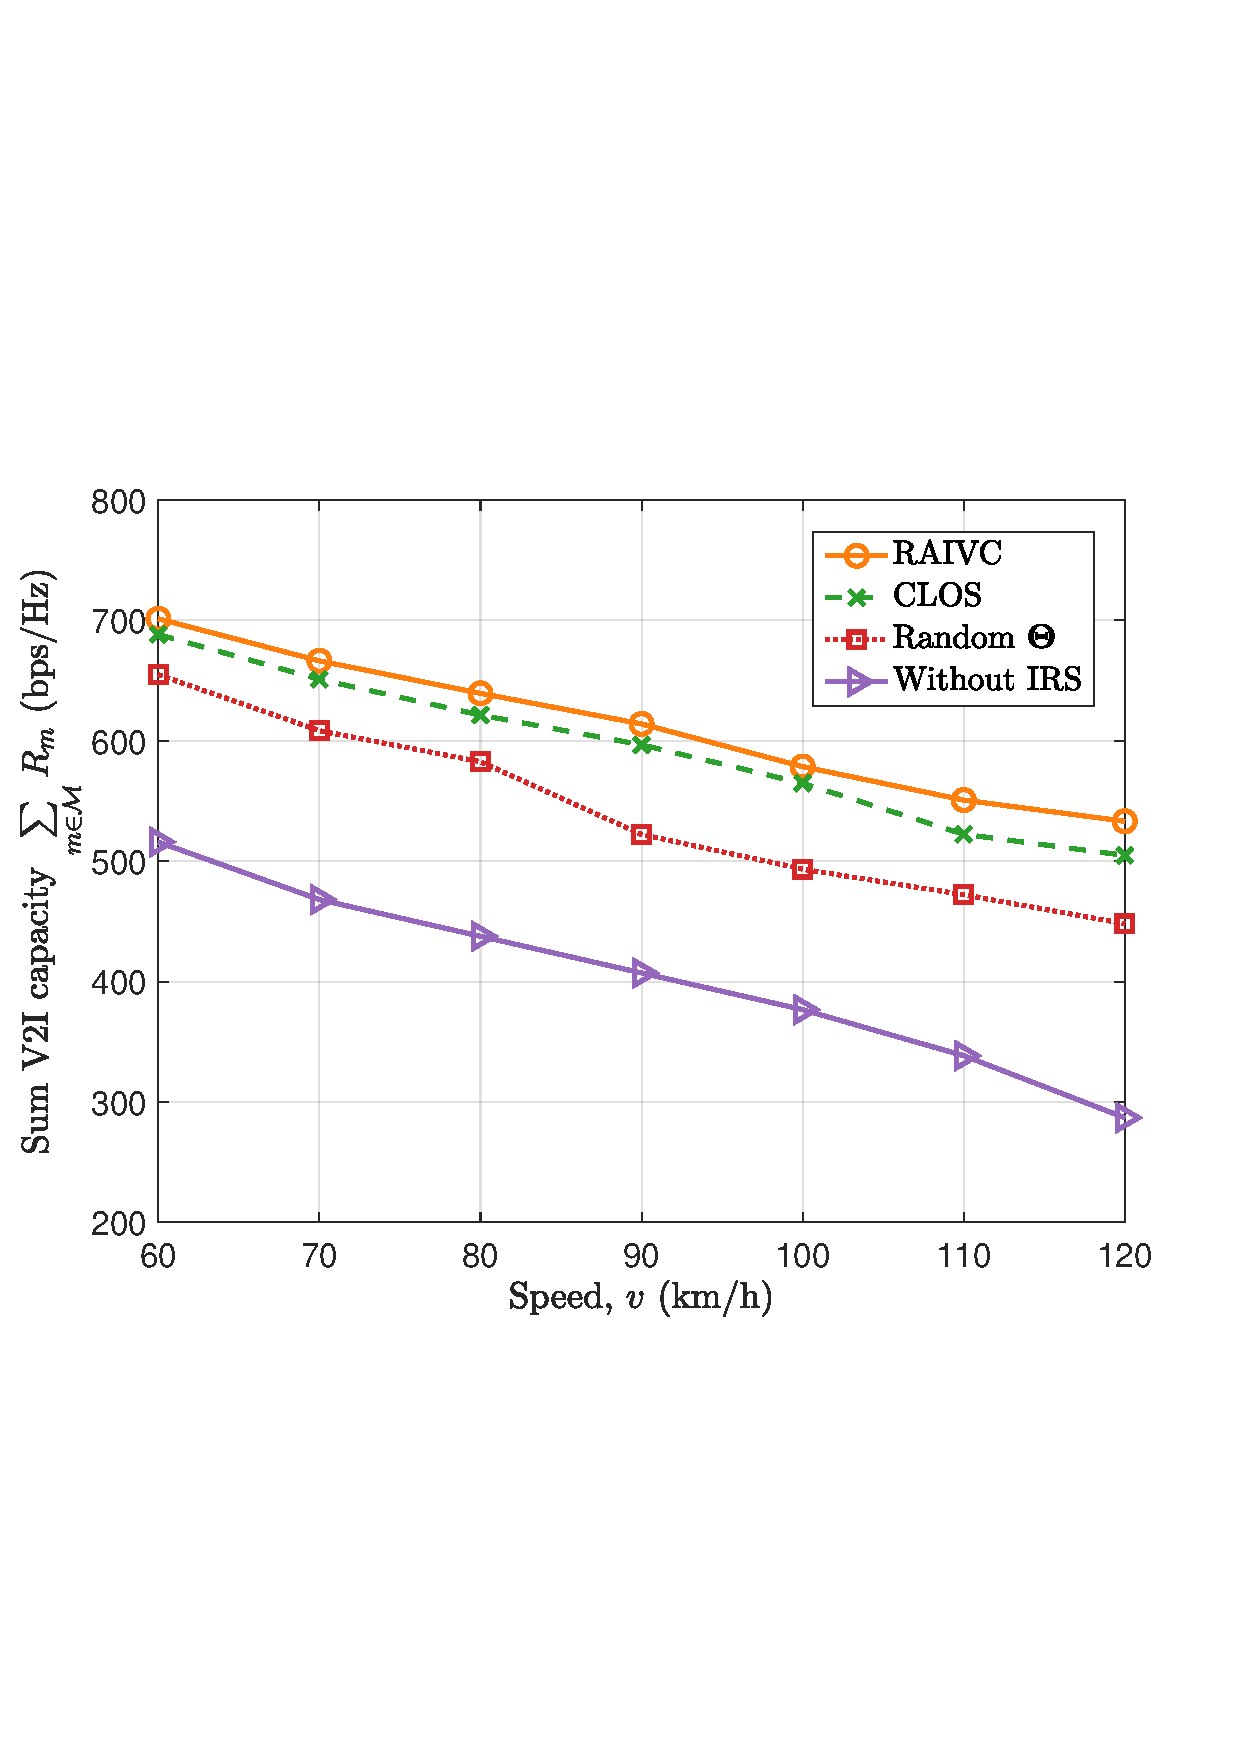
\includegraphics[width=0.8\linewidth]{Fig5.pdf}% 1\linewidth
	\caption{Sum V2I capacity versus varying vehicle speed.}
	\label{Fig5}
\end{figure}

Figure \ref{Fig5} illustrates that as the speed of the vehicle increases, the sum V2I capacity obtained by each scheme decreases, but RAIVC is still superior to three other benchmark schemems in terms of the sum V2I capacity. Meanwhile, it can be seen that with the increase of vehicle speed, the decrease of the sum V2I capacity achieved by the three schemes with IRS-aided (i.e., RAIVC, CLOS, and Random $ \bm{\Theta} $) is obviously less than that of the scheme without IRS. Specifically, when the vehicle speed varies from $60\ {\rm{km/h}}$ to $ 120\ {\rm{km/h}} $, the sum V2I capacity obtained by RAIVC decreases by 31.55\% , and obtained by without-IRS scheme decreases more, which is 79.78\%. This can be attributed to the following facts. According to our simulation settings, higher vehicle speeds result in sparse traffic, which will increase the average distance between vehicles \cite{3GPP}. In order to guarantee the SINR of V2V links, the transmission power of the D2D-V2V transmitter needs to be increased to compensate for the larger path loss of the V2V signal channel. As a result, V2I links need to tolerate greater interference from V2V links, which thus restricts the sum V2I capacity. When the IRS aids vehicular communications, the power reflected from the IRS passive reflecting elements will effectively compensate for the path loss, so that higher vehicle speed does not cause the system performance to decrease faster.


\section{Conclusions}
In this paper, we investigate the resource allocation for IRS-aided vehicular communications. Considering different QoS requirements of V2X communications, we aim to maximize the sum V2I capacity while guaranteeing the minimum SINR of V2V links. The studied problem is decomposed into two stages to solve, which yields the proposed algorithm RAIVC. Simulation results show that the proposed RAIVC algorithm is superior to other benchmark schemes and can make optimal resource allocation decisions judiciously. In terms of improving the QoS of vehicular communications, IRS-aided vehicular communications is of great significance, especially to deal with the challenges caused by complex propagation environments and high mobility. Meanwhile, significant system gain can be obtained by carefully deploying the location of the IRS. In addition, IRS-aided vehicular communications provides valuable guidelines for the practical deployment of future vehicular networks.





% if have a single appendix:
%\appendix[Proof of the Zonklar Equations]
% or
%\appendix  % for no appendix heading
% do not use \section anymore after \appendix, only \section*
% is possibly needed

% use appendices with more than one appendix
% then use \section to start each appendix
% you must declare a \section before using any
% \subsection or using \label (\appendices by itself
% starts a section numbered zero.)
%


%\appendices
%\section{Proof of the First Zonklar Equation}
%Appendix one text goes here.
%
%% you can choose not to have a title for an appendix
%% if you want by leaving the argument blank
%\section{}
%Appendix two text goes here.





% Can use something like this to put references on a page
% by themselves when using endfloat and the captionsoff option.
\ifCLASSOPTIONcaptionsoff
  \newpage
\fi



% trigger a \newpage just before the given reference
% number - used to balance the columns on the last page
% adjust value as needed - may need to be readjusted if
% the document is modified later
%\IEEEtriggeratref{8}
% The "triggered" command can be changed if desired:
%\IEEEtriggercmd{\enlargethispage{-5in}}

% references section

% can use a bibliography generated by BibTeX as a .bbl file
% BibTeX documentation can be easily obtained at:
% http://mirror.ctan.org/biblio/bibtex/contrib/doc/
% The IEEEtran BibTeX style support page is at:
% http://www.michaelshell.org/tex/ieeetran/bibtex/
%\bibliographystyle{IEEEtran}
% argument is your BibTeX string definitions and bibliography database(s)
%\bibliography{IEEEabrv,../bib/paper}
%
% <OR> manually copy in the resultant .bbl file
% set second argument of \begin to the number of references
% (used to reserve space for the reference number labels box)

\bibliographystyle{IEEEtran}
\bibliography{ref_TVTcorr}                        %ref为.bib文件名





% that's all folks
\end{document}


